\subsection{Single accelerating object in space}
 Accelerating objects like pulsars can create gravitational wave. According to general relativity, mass creates stress in space-time and thus can change the geometry of it by bending and changing the curvature. Then if this object moves, then the curvature also moves along with it. But if the object accelerates in space-time in a circular manner, then the ripples will be created in space-time which is which radiates gravitational waves. This is similar to creation of water waves when we move our finger in a circular fashion in water. So higher the mass of object and it's acceleration, stronger is the gravitational wave it produces.
 
 Such continuously spinning bodies produces continuous gravitational waves, where it's nature is sinusoidal for a longer period of time. This happens only if spin rate of this object is constant. Such gravitational waves have same frequency and amplitude, but they are not yet discovered.\\


\begin{figure}[h]
    \centering
     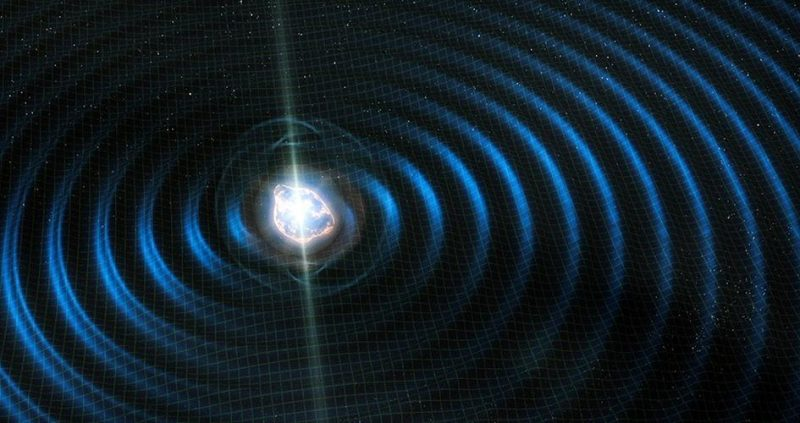
\includegraphics[height = 9cm, width = 12cm]{images.tex/continuous_gw.jpg}
    \caption{Computer simulation of Continuous gravitational wave by a pulsar \\
    \textbf{Source :-} https://earthsky.org/space/gravitational-waves-single-neutron-stars-planck-einsteinhome}
\end{figure}
